\documentclass{article}
\usepackage[T1]{fontenc}
\usepackage[utf8]{inputenc}
\usepackage{amsmath}
\usepackage{amssymb}
\usepackage{hyperref}
\usepackage{parskip} %skip the indent of a new paragraph.
\usepackage{float}
\usepackage{graphicx}
\usepackage{listings}
\lstset{language=Matlab, frame=single, breaklines=true,numbers=left, keywordstyle=\color{blue},rulecolor=\color{black},commentstyle=\color{gray}}

\usepackage{cleveref}
\usepackage{todonotes}

%% Brukes for tabeller (av likninger)
\usepackage{tabularx}
\def\tabularxcolumn#1{m{#1}}

\newcommand{\TODO}[1]{\todo[inline]{#1}}
\newcommand{\mbf}[1]{\mathbf{#1}} % Arg 1 is bold (in math environment)
\newcommand{\partialderiv}[2]{\frac{\partial{#1}}{\partial{#2}}} % prints partial derivative as a fraction

\title{Linear Systems TTK4115 - Helicopter Lab Report}
\author{Bern Johan Damslora -- 759477 \\ Didrik rokhaug -- 759528}
\date{\today}

\begin{document}

\begin{titlepage}
    %\maketitle
    %\rule{\linewidth}{0.5mm}
    \begin{center}
    	\large
    	Linear Systems TTK4115
    \end{center}
    \vspace{\fill}
    \rule{\linewidth}{0.5mm}
    \begin{center}
    	\huge
    	Helicopter Lab Report
    \end{center}
	\rule{\linewidth}{0.5mm}
	\vspace{\fill}

	%\begin{center}
    %	\huge
    %	Bern Johan Damslora -- 759477 \\ Didrik rokhaug -- 759528
    %\end{center}
    \begin{table}[H]
    	\centering
    	\large
    	\begin{tabular}{rl}
    		\textbf{Bernt Johan Damslora} & (nr. 759477) \\
    		\textbf{Didrik Rokhaug} &  (nr. 759528)
    	
    	\end{tabular}
    \end{table}
    \vspace{\fill}
    \begin{center}
    	\large
    	\today
    \end{center}
	\vspace{\fill}
    \begin{figure}[H]
    \centering
    
\includegraphics[width=0.5\textwidth]{images/logontnu_eng}
    \end{figure}
    \thispagestyle{empty}
\end{titlepage}

%\section*{Table of contents} 
\tableofcontents
\thispagestyle{empty} %Avoid page numbering on the table of contents
\newpage    

\setcounter{page}{1}
\section{Part 1: Mathematical modeling}
To find a model of the system we started with Newton's 2nd law for rotation, which states that
\begin{equation} \label{eq:N2rot}
\sum \tau = J \alpha
\end{equation}
where $\tau$ is the external torque, $J$ is the moment of inertia, and $\alpha$ is the angular acceleration. Using this for each of the three axis gives
\begin{subequations}
  \begin{align}
    J_p\ddot{p} &= L_{1}V_{d} \label{eq:ulinsysp}\\
    J_e\ddot{e} &= L_{2} \cos(e) + L_3 V_s \cos(p) \label{eq:ulinsyse}\\
    J_\lambda \ddot{\lambda} &= L_4 V_s \cos(e) \sin(p) \label{eq:ulinsysl}
  \end{align}
  \label{eq:ulinsys}
\end{subequations}
where 
\begin{subequations}
	\begin{align*}
		L_1 &= K_f l_p\\
		L_2 &= (m_c l_c - 2 m_p l_h)g\\
		L_3 &= K_f l_h
	\end{align*}
\end{subequations}

As the model in \cref{eq:ulinsys} is non-linear we need to linearize the model to be able to design a linear controller. To do this we need a point to linearize around. For this we use $(p^*, e^*, \lambda^*)^T = (0, 0, 0)^T$. We also need to find the voltages $V_s^*$ and $V_d^*$ that makes $(p^*, e^*, \lambda^*)^T$ an equilibrium. Setting \cref{eq:ulinsysp} and \cref{eq:ulinsyse} to zero gives

\begin{subequations}
	\begin{align*}
		V_d^* &= 0\\
		V_s^* &= -\frac{L_2}{L_3}
	\end{align*}
\end{subequations}

The next thing we did was a coordinate transform, to simplify the model of the system. The new states are $ (\tilde p, \tilde e, \tilde \lambda)^T = (p, e, \lambda)^T - (p^*, e^*, \lambda^*)^T $ and the new inputs are $(\tilde V_s, \tilde V_d)^T = (V_s, V_d)^T - (V_s^*, V_d^*)^T $. This gives the system

\begin{subequations}
	\begin{align}
		\ddot{\tilde p} &= \frac{L_1}{J_p} \tilde V_d\\
		\ddot{\tilde e} &= \frac{L_2}{J_e} \cos \tilde e + (L_3 \tilde V_s - L_2) \cos \tilde p\\
		\ddot{\tilde \lambda} &= %\todo{sjekk notater til Bernt Johan om utrykket står der}
	\end{align}
	\label{eq:transformertulinsys}
\end{subequations}

Now that the system is on a nice form, we can linearize it. This gives us a system on the form $ \dot{\mbf{x}} = \mbf{A} \mbf{x} + \mbf{B} \mbf {u} $, where the matrices is given by
	
\begin{subequations}
	\begin{align}
		\mbf{A} &= \begin{bmatrix}
			\partialderiv{\ddot{\tilde{p}}}{\tilde p} = 0 & \partialderiv{\ddot{\tilde p}}{\tilde e} = 0 & \partialderiv{\ddot{\tilde p}}{\tilde \lambda} = 0\\[0.3em]
			\partialderiv{\ddot{\tilde{e}}}{\tilde p} = 0 & \partialderiv{\ddot{\tilde{e}}}{\tilde e} = 0 & \partialderiv{\ddot{\tilde{e}}}{\tilde \lambda} = 0\\[0.3em]
			\partialderiv{\ddot{\tilde \lambda}}{\tilde p} = -\frac{L_2}{J_{\lambda}} & \partialderiv{\ddot{\tilde \lambda}}{\tilde e} = 0 & \partialderiv{\ddot{\tilde \lambda}}{\tilde \lambda} = 0
		\end{bmatrix} \\
		\mbf{B} &= \begin{bmatrix}
			\partialderiv{\ddot{\tilde p}}{\tilde V_s} = 0 & \partialderiv{\ddot{\tilde p}}{\tilde V_d} = \frac{L_1}{J_p}\\[0.3em]
			\partialderiv{\ddot{\tilde e}}{\tilde V_s} = \frac{L_3}{J_e} & \partialderiv{\ddot{\tilde e}}{\tilde V_d} = 0\\[0.3em]
			\partialderiv{\ddot{\tilde \lambda}}{\tilde V_s} = 0 & \partialderiv{\ddot{\tilde \lambda}}{\tilde V_d} = 0
		\end{bmatrix}
	\end{align}
	\label{eq:linearisert}
\end{subequations}

Writing out \cref{eq:linearisert} we get

\begin{subequations}
	\begin{align}
		\ddot{\tilde p} &= \frac{L_1}{J_p} \tilde V_d = K_1 \tilde V_d\\
		\ddot{\tilde e} &= \frac{L_3}{J_e} \tilde V_s = K_2 \tilde V_s\\
		\ddot{\tilde \lambda} &= -\frac{L_2}{J_{\lambda}} \tilde p = K_3 \tilde p
	\end{align}
\end{subequations}


\section{Part 2: Monovariable Control}
\section{Part 3: Multivariable Control}
\subsection{Problem 1}
The system can be described as
\begin{subequations}
\begin{equation}
	\mbf{\dot x = Ax + Bu}
\end{equation}
where \\
	\begin{tabularx}{\textwidth}{XX}
	 \begin{equation}
	   \mbf{x} = \begin{bmatrix}
	   	\tilde p \\ \dot{\tilde p} \\ \dot{\tilde e}
	   \end{bmatrix}
	 \end{equation}
	 &
	 \begin{equation}
	   \mbf{u} = \begin{bmatrix}
	   	\tilde {V_s} \\ \tilde {V_d}
	   \end{bmatrix}
	 \end{equation}
	\\
		\begin{equation}
			\mbf{A} = \begin{bmatrix}
				0 & 1 & 0 \\ 0 & 0 & 0 \\ 0 & 0 & 0
			\end{bmatrix}
		\end{equation}
		&
		\begin{equation}
			\mbf{B} = \begin{bmatrix}
				0 & 0 \\ 0 & K_1 \\ K_2 & 0
			\end{bmatrix}
		\end{equation}
	\end{tabularx}
\end{subequations}

\subsection{Problem 2}
We verified the controllability of the system by checking that the controllability matrix $\mathcal{C}$ has full rank, as shown in \cref{eq:c}.
\begin{equation}
	\mathcal{C} = \begin{bmatrix}
		\mbf{B} & \mbf{AB} & \mbf{A^2 B}
	\end{bmatrix} = \begin{bmatrix}
		0 & 0 & 0 & K_1 & 0 & 0\\ 0 & K_1 & 0 & 0 & 0 & 0\\ K_2 & 0 & 0 & 0 & 0 & 0
	\end{bmatrix} \label{eq:c}
\end{equation}
The feed-forward matrix $\mbf{P}$ was defined as \todo{gjorde vi noen utregninger her? Kanskje sitere forelesningen/boken/?????}
\begin{equation}
	\mbf{P = (C (B K-A)^{-1} B)^{-1}}
\end{equation}
and computed by MATLAB after $\mbf{K}$.

We then set out to define the weighting matrices $\mbf{Q}$ and $\mbf{R}$. We used Bryson's rule (setting each diagonal weight to the inverse square of the maximum allowable error($\mbf{Q}$) or input($\mbf{R}$)) as a starting point. Keeping the form of Bryson's rule, we adjusted the ``maximum allowable values'' until results were satisfactory. We ended up with Q and R matrices shown in \cref{eq:QR}.

\begin{subequations}
	\begin{tabularx}{\textwidth}{XX}
	 \begin{equation}
	   \mbf{Q} = \begin{bmatrix}
	   	\frac{\pi}{4}^{-2} & 0 & 0 \\
	   	0 & 2\pi^{-2} & 0 \\
	   	0&0& \frac{\pi}{5}^{-2}
	   \end{bmatrix}
	 \end{equation}
	 &
	 \begin{equation}
	   \mbf{R} = \begin{bmatrix}
	   	9^{-2} & 0 \\
	   	0 & 9^{-2}
	   \end{bmatrix}
	 \end{equation}
	\end{tabularx}
	\label{eq:QR}
\end{subequations}

Keeping the units in mind, these values make sense. The allowable pitch error is 1/8th of a circle, the allowable pitch rate ``error'' is 1 revolution per second, and the allowable elevation rate error is 1/10th of a revolution per second. The allowable inputs are 9 volts, which makes sense, considering that the motors saturate at a sum or difference of 10 volts.

Finally, the $\mbf{K}$ was calculated by tha MATLAB function \verb+K = lqr(A,B,Q,R)+.
\TODO{Legg inn faktisk K og P?}

\subsection{Problem 3}
We add the integrated states and get the augmented system with new matrices, described by the state space model
\begin{subequations}
\begin{equation}
	\mbf{\dot x = Ax + Bu}
\end{equation}
where \\
	\begin{tabularx}{\textwidth}{XX}
	 \begin{equation}
	   \mbf{x} = \begin{bmatrix}
	   	\tilde p \\ \dot{\tilde p} \\ \dot{\tilde e} \\ \int_0^t{\tilde p} \\ \int_0^t{\dot{\tilde e}}
	   \end{bmatrix}
	 \end{equation}
	 &
	 \begin{equation}
	   \mbf{u} = \begin{bmatrix}
	   	\tilde {V_s} \\ \tilde {V_d}
	   \end{bmatrix}
	 \end{equation}
	\\
		\begin{equation}
			\mbf{A} = \begin{bmatrix}
				0 & 1 & 0 & 0 & 0 \\ 0 & 0 & 0 & 0 & 0 \\ 0 & 0 & 0 & 0 & 0 \\ 1 & 0 & 0 & 0 & 0 \\ 0 & 0 & 1 & 0 & 0
			\end{bmatrix}
		\end{equation}
		&
		\begin{equation}
			\mbf{B} = \begin{bmatrix}
				0 & 0 \\ 0 & K_1 \\ K_2 & 0
			\end{bmatrix}
		\end{equation}
	\end{tabularx}
\end{subequations}
% Part 4
\section{Part 4: state estimation}
\subsection{Problem 1}
To get a better controller we want to use an observer to estimate some of the states, rather than using the derivative of the output. To make the observer we need a model of the system with all the states, both measured and estimated, and those we want to estimate. This model can be written as

\begin{subequations}
	\begin{align*}
		\mbf{\dot x} &= \mbf{A}\mbf{x} + \mbf{B}\mbf{u}\\
		\mbf{y} &= \mbf{C}\mbf{x}
	\end{align*}
\end{subequations}

where the vectors $\mbf{x}$, $\mbf{u}$ and $\mbf{y}$, and the matrices $\mbf{A}$, $\mbf{B}$ and $\mbf{C}$ are given by

\begin{subequations}
	\begin{align}
		\mbf{x} &= \begin{bmatrix}
			\tilde p\\
			\dot{\tilde p}\\
			\tilde e\\
			\dot{\tilde e}\\
			\tilde \lambda\\
			\dot{\tilde \lambda}
			\end{bmatrix}, 
		\mbf{u} = \begin{bmatrix}
			\tilde V_s\\
			\tilde V_d
			\end{bmatrix} \text{and} \ 
		\mbf{y} = \begin{bmatrix}
			\tilde p\\
			\tilde e\\
			\tilde \lambda
			\end{bmatrix}\\
		\mbf{A} &= \begin{bmatrix}
			0 & 1 & 0 & 0 & 0 & 0\\
			0 & 0 & 0 & 0 & 0 & 0\\ 
			0 & 0 & 0 & 1 & 0 & 0\\
			0 & 0 & 0 & 0 & 0 & 0\\
			0 & 0 & 0 & 0 & 0 & 1\\
			K_3 & 0 & 0 & 0 & 0 & 0
			\end{bmatrix}\\
		\mbf{B} &= \begin{bmatrix}
			0 & 0\\
			0 & K_1 &\\
			0 & 0\\
			K_2 & 0\\
			0 & 0\\
			0 & 0	
			\end{bmatrix}\\
		\mbf{C} &= \begin{bmatrix}
			1 & 0 & 0 & 0 & 0 & 0\\
			0 & 0 & 1 & 0 & 0 & 0\\
			0 & 0 & 0 & 0 & 1 & 0
			\end{bmatrix}
	\end{align}
\end{subequations}

\subsection{Problem 2}
Using the MATLAB functions \texttt{obsv(sys)} and \texttt{rank(matrix)} we found that the observability matrix $\mathcal{O}$ have a $\text{rank} = 6$, which is the same as the systems dimension. This means that the system is observable.

We then used the new model to make a linear observer on the form $\mbf{\dot{\hat x}} = \mbf{A}\mbf{\hat x} + \mbf{B}\mbf{u} + \mbf{L} (\mbf{y}-\mbf{C}\mbf{\hat x})$. The observer gain matrix $L$ was found by using the function \texttt{place(A', C', poles).'}. For the controller with integral effect the poles we chose were placed in a fan with a opening of \todo{insert angle here}, and a radius of $20 \cdot r_0$ where $r_0$ is the absolute value of the largest pole of the closed loop system $\mbf{\dot x} = (\mbf{A} - \mbf{B} \mbf{K}) \mbf{x}$. The way we ended up with these poles were by following the recommendations from the lectures of placing them in a fan with a radius sufficiently larger than the absolute value of the largest pole of the cosed loop system, and then trying different radii until we found one that gave a satisfying response. For the controller without integral effect we followed the same procedure, and ended up with the same $\mbf{L}$ matrix. \todo[inline]{Er det godt nok forklart hvordan vi fant og plaserte polene?} 


As the observer does not simply differentiate the output, but also uses it's knowledge of the input it is able to filter out some of the noise. A fast observer will give an accurate estimate, whereas a slow observer will filter out more noise. This means that these benefits needs to be balanced when choosing the poles of the observer. As we can see from \cref{fig:pest}, \cref{fig:pdest}, \cref{fig:eest} and \cref{fig:edest} the observer follows the real values closely, while filters out most of the noise.

\begin{figure}[H]
	\centering
	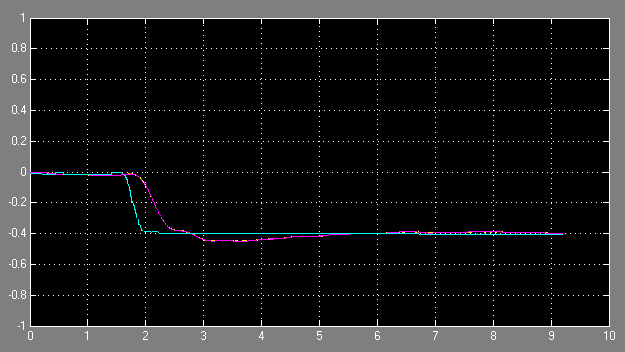
\includegraphics[width=0.95\textwidth]{images/est_med_int/p_est.png}
	\caption{Pitch. Yellow = measurement, red = estimate, blue = reference}
	\label{fig:pest}
\end{figure}
\begin{figure}[H]
	\centering
	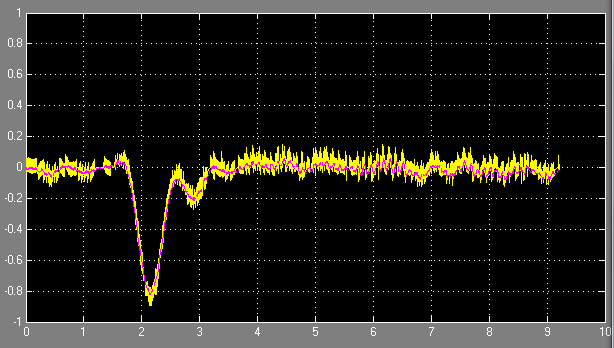
\includegraphics[width=0.95\textwidth]{images/est_med_int/pd_est.png}
	\caption{Pitch rate. Yellow = measurement, red = estimate}
	\label{fig:pdest}
\end{figure}
\begin{figure}[H]
	\centering
	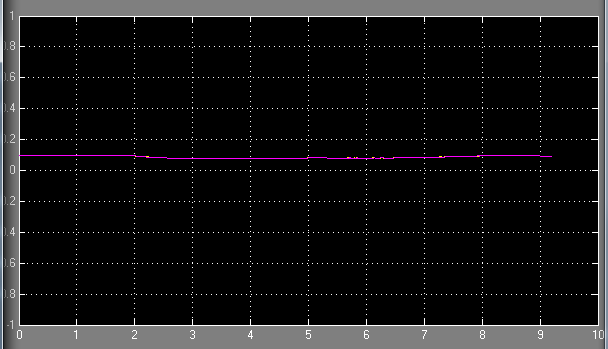
\includegraphics[width=0.95\textwidth]{images/est_med_int/e_est.png}
	\caption{Elevation. Yellow = measurement, red = estimate}
	\label{fig:eest}
\end{figure}
\begin{figure}[H]
	\centering
	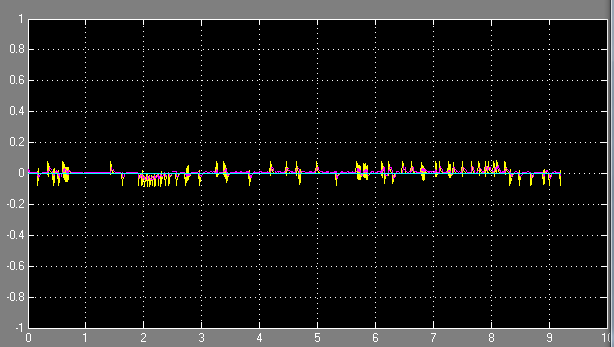
\includegraphics[width=0.95\textwidth]{images/est_med_int/ed_est.png}
	\caption{Elevation rate. Yellow = measurement, red = estimate, blue = reference}
	\label{fig:edest}
\end{figure}


\subsection{Problem 3}
If we only measure $\tilde p$ and $\tilde e$ we we get the following $\mbf{A}$ and $\mbf{C}$ matrices:

\begin{subequations}
	\begin{align}
		\mbf{A} &= \begin{bmatrix}
			0 & 1 & 0 & 0 & 0 & 0\\
			0 & 0 & 0 & 0 & 0 & 0\\
			0 & 0 & 0 & 1 & 0 & 0\\
			0 & 0 & 0 & 0 & 0 & 0\\
			0 & 0 & 0 & 0 & 0 & 1\\
			K_3 & 0 & 0 & 0 & 0 & 0
		\end{bmatrix}\\
		\mbf{C} &= \begin{bmatrix}
			1 & 0 & 0 & 0 & 0 & 0\\
			0 & 0 & 1 & 0 & 0 & 0\\
			0 & 0 & 0 & 0 & 1 & 0
		\end{bmatrix}
	\end{align}
\end{subequations}

If we calculate the observer matrix $\mathcal{O}$ we get that the rank is 6, which means that the system is observable. However trying to control the system we found that the observer were too bad to be used to control the helicopter. The reason for the bad estimates is that we control the pitch and pitch rate which are not measured. This means that we try to estimate a states that are the second and third derivative of one of the states that we measure. This means that even though it is theoretically possible to control the system, it is very hard to make a good controller that works well on the real system. Another reason why the estimates are poor are because the estimator is based on a linear model, while the real system is non-linear. Even though we weren't able to control the system, we were at least able to get the estimator stable, and when we hold the helicopter down, all the estimates go towards the right values.

\newpage
%\addcontentsline{toc}{section}{References} %uncomment if you want the references included in the table of content
\bibliographystyle{plain}
\bibliography{ref.bib}


\end{document}
